\documentclass{article}
\usepackage{graphicx}
\usepackage{listings}
\graphicspath{ {images/} }

 \pagenumbering{arabic}
 \usepackage{array}
 





\begin{document}


\includegraphics[width=10cm, height=5cm]{logo} \break \break

\centering {\textbf{Computer Science and Engineering} }\\

 \centering{A.A. 2016/2017} \\
\centering{Software Engineering 2 Project:} \\

\centering{\textbf{ Power\&Joy} }\break



\centering{\textbf{\large{Integration  Test  Plan  Document }} }\break \break

\centering{November 11, 2016 }\break





\begin{flushright}


Prof. Luca Mottola\break 
Joshua Nicolay Ortiz Osorio \ Mat: 806568 \\
Michelangelo Medori \ Matr: 878025

\end{flushright}

\newpage

\centering {\textbf{Index}} \\    %INDEX
\begin{enumerate}

\item Introduction




\begin {enumerate}
\item [1.1] Revision History
\item [1.2] Purpose and Scope
\item [1.3] List of Definitions and Abbreviations 
\item [1.4] List of Reference Documents

\end{enumerate}

\item Integration Strategy 
\begin {enumerate}
\item [2.1] Entry Criteria
\item [2.2] Elements to be Integrated 
\item [2.3] Integration Testing Strategy
\item [2.4] Sequence of Component/Function Integration 
\begin {enumerate}
\item [2.4.1] Software  Integration  Sequence
\item [2.4.2] Subsystem  Integration  Sequence
\end {enumerate} 

\end {enumerate} 


\item Individual Steps and Test Description



\item Tools and Test Equipment Required  



\item Program Stubs and Test Data Required 



\item Effort Spent 

\end{enumerate}

\newpage   			
\begin{flushleft}  

  \section{Introduction}	% 1)INTRODUCTION
  \subsection{Revision History} 	% 1.1)REVISION HISTORY
  
  \begin{center}
    \begin{tabular}{ | p{2cm} | p{2cm} |  p{7 cm} | p{4cm} |}
    \hline
    \textbf{Version} &  \textbf{Date} & \textbf{Author(s)} & \textbf{Summary}  \\ 
    \hline
    
    1.0 & 10/01/2017 & Joshua Nicolay Ortiz Osorio and Michelangelo Medori & initial release
     \\ 
  \hline
  
  
  2.0 & 14/01/2017 & Joshua Nicolay Ortiz Osorio and Michelangelo Medori & completed sections 5 and 6, small changes to section 3\\
  \hline
  
    \end{tabular}
\end{center}
	
  \subsection{Purpose and Scope}		% 1.2)PURPOSE AND SCOPE
  This is the  Integration Testing Plan Document for the Power\&Joy car sharing management system.
  The purpose of this document is to describe in a detailed way the organisation of the integration test activity, which involves all the components that are going to be assembled to build the system\\
  In the following sections we are going to provide:\\
  \begin{itemize}
     \item In section 2.1 we describe the criteria that must be met by the project status before integration testing of the outlined elements may begin
  
  \item In section 2.2 we provide a list of the subsystems and their subcomponents involved in the integration testing  activity 

    \item  In section 2.3 we provide a description of the integration testing approach
     \item The sequence in which components and subsystems will be integrated is described in sections 2.4.1 and 2.4.2
      \item  Section 3 contains a description of the planned testing activities for each integration step, including their input data and the expected output
       \item  A list of all the tools that will have to be employed during the testing activities, together with a description of the operational environment in which the tests will be executed can be found in section 4 and 5
       
  \end{itemize}
  
  
  \subsection{List of Definitions and Abreviations }		% 1.3)LIST OF DEFINITIONS AND ABREVATIONS
  \subsubsection{Definitions}
  \begin{itemize}
  \item Subcomponent: each of the low level components realising the functionalities of a subsystem.
  \item Subsystem: a high-level functional unit of the system.
  \end{itemize}
  
  \subsubsection{Acronyms}
    \begin{itemize}
  \item RASD : Requirements Analysis and Specifications Document
  
  \item DD: Design Document
  \item ITPD:  Integration Test Plan Document
  \item DBMS: Data Base Management System
  \item GPS: Global Positioning System
  \item UI: User Interface
  \item Notification system: a combination of software and hardware that provides a means of delivering a message to a set of recipients
  \item User : someone who registered into the system and can can access the system in order to reserve and ride a car  
  \item Operator: Someone who provides assistance to users, works in one of the stations
  \item Station: place where operators work
  \item CarId: Unique identifier for every car
  \item ReservationId: Unique identifier for every Reservation 
  \item RideId: Unique identifier for every Ride
  \item UserId: Unique identifier for every User
  \item OperatorId: Unique identifier for every Operator
  
  \end{itemize}
  
 
  
  \subsection{List of Reference Documents}		% 1.4)LIST OF REFERENCE DOCUMENTS
  \begin{itemize}
   \item Assignment AA 2016-2017
    \item Requirements analysis and Specifications Document (RASD)
     \item design Document (DD)
      \item Integration Test Plan Example.pdf
      \item Integration testing example document.pdf
  \end{itemize}
  
  
  \newpage
  \section{Integration Strategy }  		% 2)INTEGRATION STRATEGY
   \subsection{Entry Criteria}		% 2.1)ENTRY CRITERIA
   Before the Integration test can start, there are several conditions about the current state of the project workflow  that should be verified. First of all the RASD and DD need to be fully completed and available.
   Furthermore, the test should only start if the components to be integrated have reached the completion levels  described below:
   
   \begin{itemize}
   \item 100\% for the Data Access Utility
   \item At least 90\%  for the Car sharing management system
   \item At least 75\% for the System Administration and Account Management subsystems
   \item At least 60\% for the client applications
   
   
   
   
   \end{itemize}
   
   These percentages are to be considered at the beginning of the integration test and take into account also the order in which the components need to be integrated and the time needed for the integration test. For any component, the minimum percentage that allows it to be considered for integration is 90\%
   \subsection{Elements to be Integrated }		% 2.2)ELEMENTS TO BE INTEGRATED
   In this paragraph we are going to describe the structure of the Power\&Joy system in terms of its subsystems and the subcomponents they are made of.  The subsystems  are the following:
   \begin{itemize}
   \item Car sharing management system 
   \item System administration 
   \item Account Management system
   \item Data Access Utilities
   \item DBMS
   \item Mapping Service
   \item Notification system
   \item Remote services interface
   \end{itemize}  
   
   The Car sharing management system is composed by the following lower level subcomponents:
      \begin{itemize}
   \item Reservation management
   \item Ride Management 
   \item Location management 
   \item Car management 
   \item Issues management 
   \end{itemize}
   
   These subcomponents strongly rely on each other, and their precise integration is necessary to build all the functionalities the Car sharing management system. 
   
   The account management and system administration subsystems, are two collections of subcomponents that do not interact with each other, but their functionalities fall under the same field. The subcomponents constituting these subsystems are the following:
   For the Administration subsystem:
   \begin{itemize}
   \item The operator management 
   \item The Station location 
   \item The service statistics 
   \item Discounts\&penalities management 
   \item Payment management
   \end{itemize}
   
   The account management subsystem takes care both of the users and the operators accounts, registrations and logins, and it is made by the following subcomponents::
   \begin {itemize}
   \item The Login management
   \item The password retrieval management
   \item The registration management 
   \item The settings management 
   \end{itemize}
    
   
   Once the lower level subcomponents have successfully been integrated, we can think about integrating the resulting high level subsystems together in order to have the Power\&Joy System.
   The data access utilities is an atomic high level component , while all the other high level components (DBMS, mapping service, remote services interface and the notification system) already exist and are just integrated in order to provide the system with more functionalities.
   
   
   
\newpage   
   \subsection{Integration Testing Strategy}		% 2.3)INTEGRATION TESTING STRATEGY
   The strategy we are going to use to perform the integration tests is mainly the bottom-up approach, that consists on integrating  those components which do not functionally depend on other components of the system first, and proceeding with all the other components, as soon as the ones they depend on are already been successfully integrated. \\ 
   This approach is very reliable, since the final system is going to be built from subsystems which have already been tested and knowing that they work properly. This implies that in case errors occur, they only affect the current step of the integration, and not the integration already performed.\\
    It is appropriate and efficient that the components to be integrated are actually developed with a bottom-up approach as well, which means that the integration tests can be performed as soon as the components they involve are fully developed. The fact that many components are often functionally independent from each other, also lets us choose the ones to integrate first, enabling us to follow a critical-first approach as well, which means that we can start integrating the highest risk subsystems, that actually are the ones that take care of the main functionalities of the system (i.e. its management subsystem, which is composed by the reservation management, ride management, issues management, location management and car management subcomponents, as described above) before concentrating with all the other components, that take care of minor functionalities. \\
    We also have some components that are commercial components, and thus come already fully developed and working and can be used in a bottom up approach already at the beginning of the integration test. These components are DBMS, mapping service, remote service interface and notification system.
   
   \newpage
   
   
   
   
   \subsection{Sequence of Component/Function Integration}		% 2.4)SEQUENCE OF COMPONENTS/FUNCTION INTEGRATION
   
In this section we?re going to describe the order of integration (and integration testing) of the various components and subsystems of Power\&Joy system. 
   As a notation, given C1 and C2 two components/subcomponent/subsystems, an arrow from C1 to C2 means that C2 requires C1's subcomponents  to have  been fully implemented, integrated and tested and C1 to properly work in order for C2 to function .\\
   
    
   
   
   
  
  \subsubsection{Software  Integration  Sequence}		% 2.4.1)SOFTWARE INTEGRATION SEQUENCE
  Following the bottom up approach, we are going to describe in which order the subcomponents are to be integrated and tested.
    \break \break
  
  \textbf{Data Access Utilities} \\
  The first two elements to be integrated are the Data Access Utilities and the Database Management System components, since every other component relies on Data Access Utilities to perform queries on the underlying database.\\
   \vspace{1cm}
  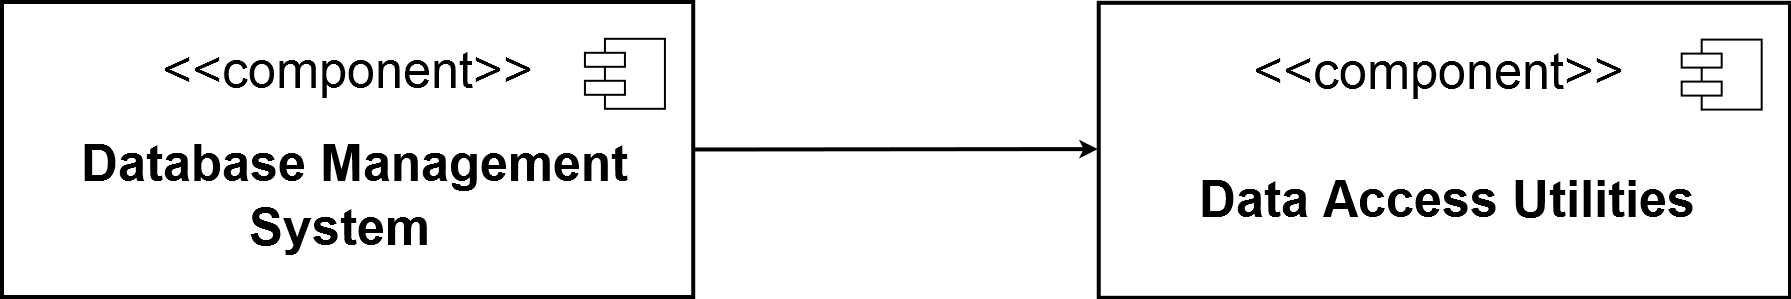
\includegraphics[scale=0.2]{Diagramma2}
    \break \break
    
    \textbf{Car sharing management system}\\
    Now we are going to describe how to integrate the subcomponents of the Car sharing management system, which is the core of the Power\&Joy System. 
    First we want the Reservation management subcomponent to be integrated with the Data Access Utilities and the Notification System:\\
 \vspace{1cm}
  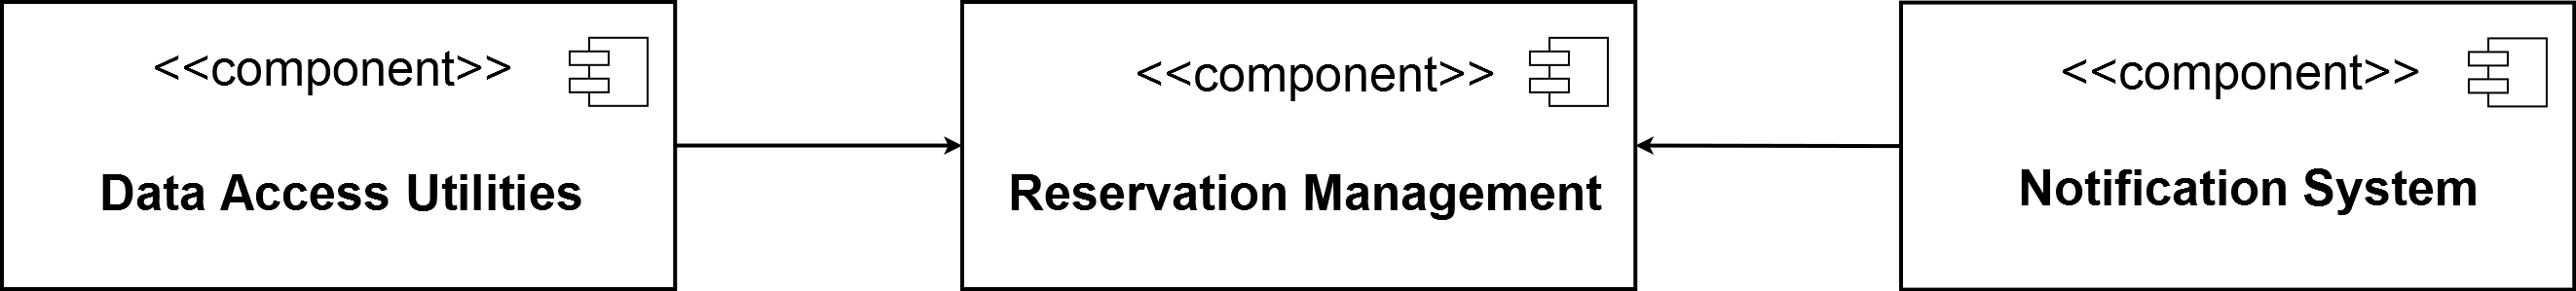
\includegraphics[scale=0.15]{Diagramma3}
    
    \newpage
    Then we need the Ride Management subcomponent to be integrated with the Data Access utilities and the Notification System: \\
    \vspace{1cm}
  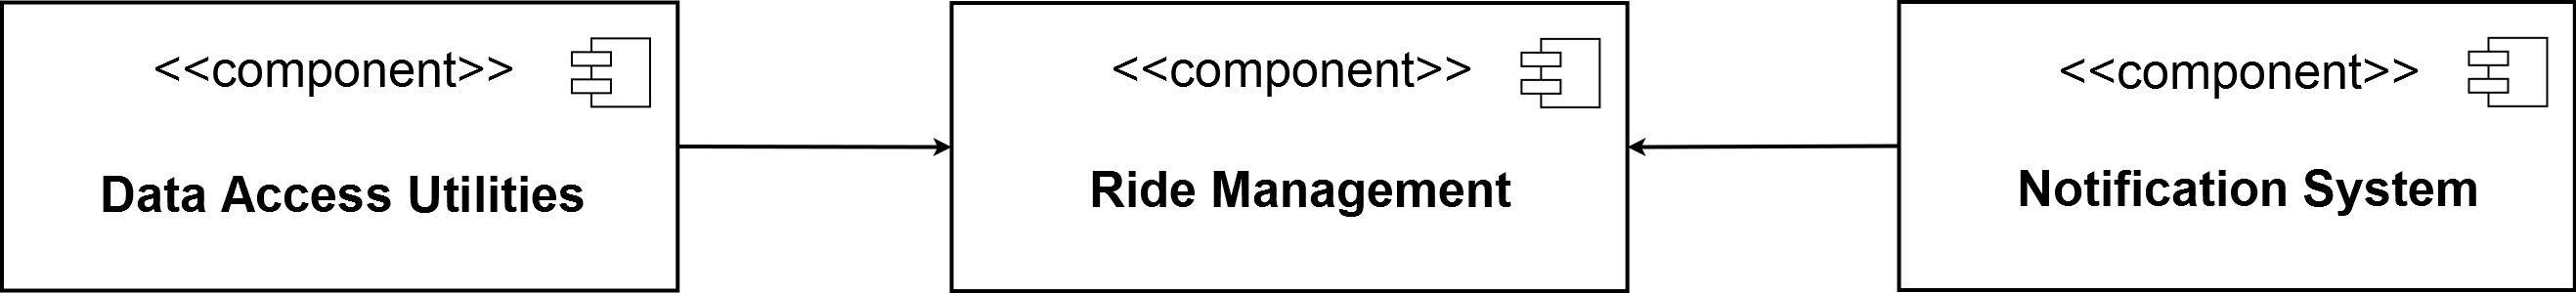
\includegraphics[scale=0.15]{Diagramma4}
    \break \break
    
    The same is for the Issues manager, to be integrated with the Data Access Utilities and the Notification System:\\
 \vspace{1cm}
  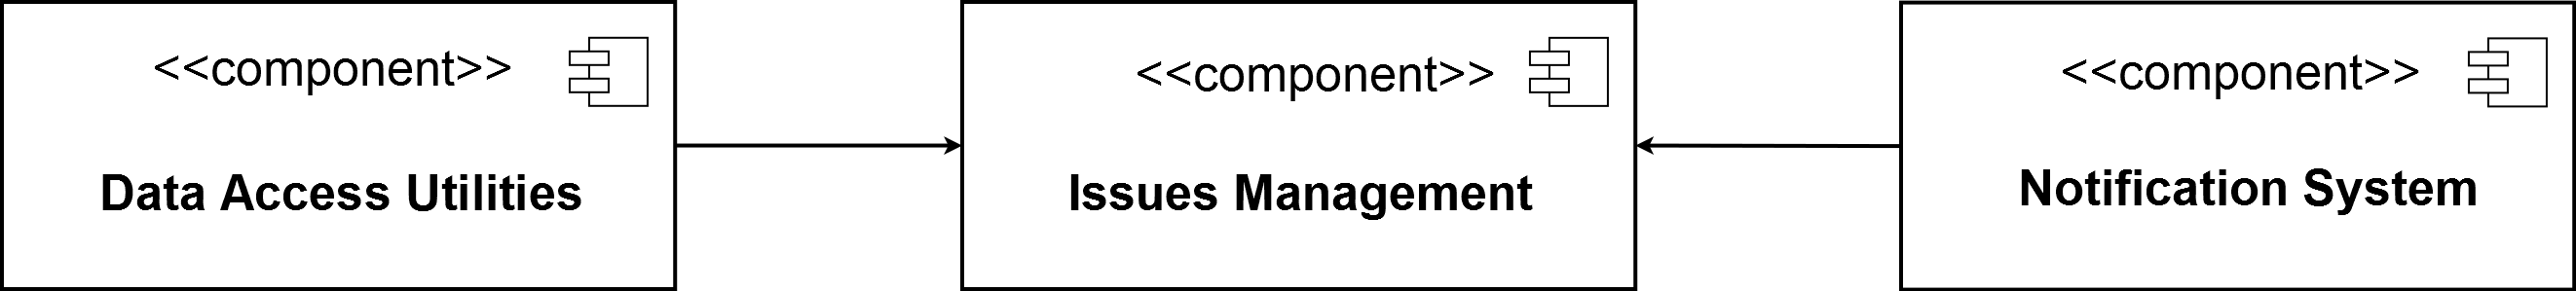
\includegraphics[scale=0.15]{Diagramma10}
    \break \break
    
    Finally, we need to integrate the car Management subcomponent with the notification Service, Data Access utilities and Mapping Service:\\
     \vspace{1cm}
  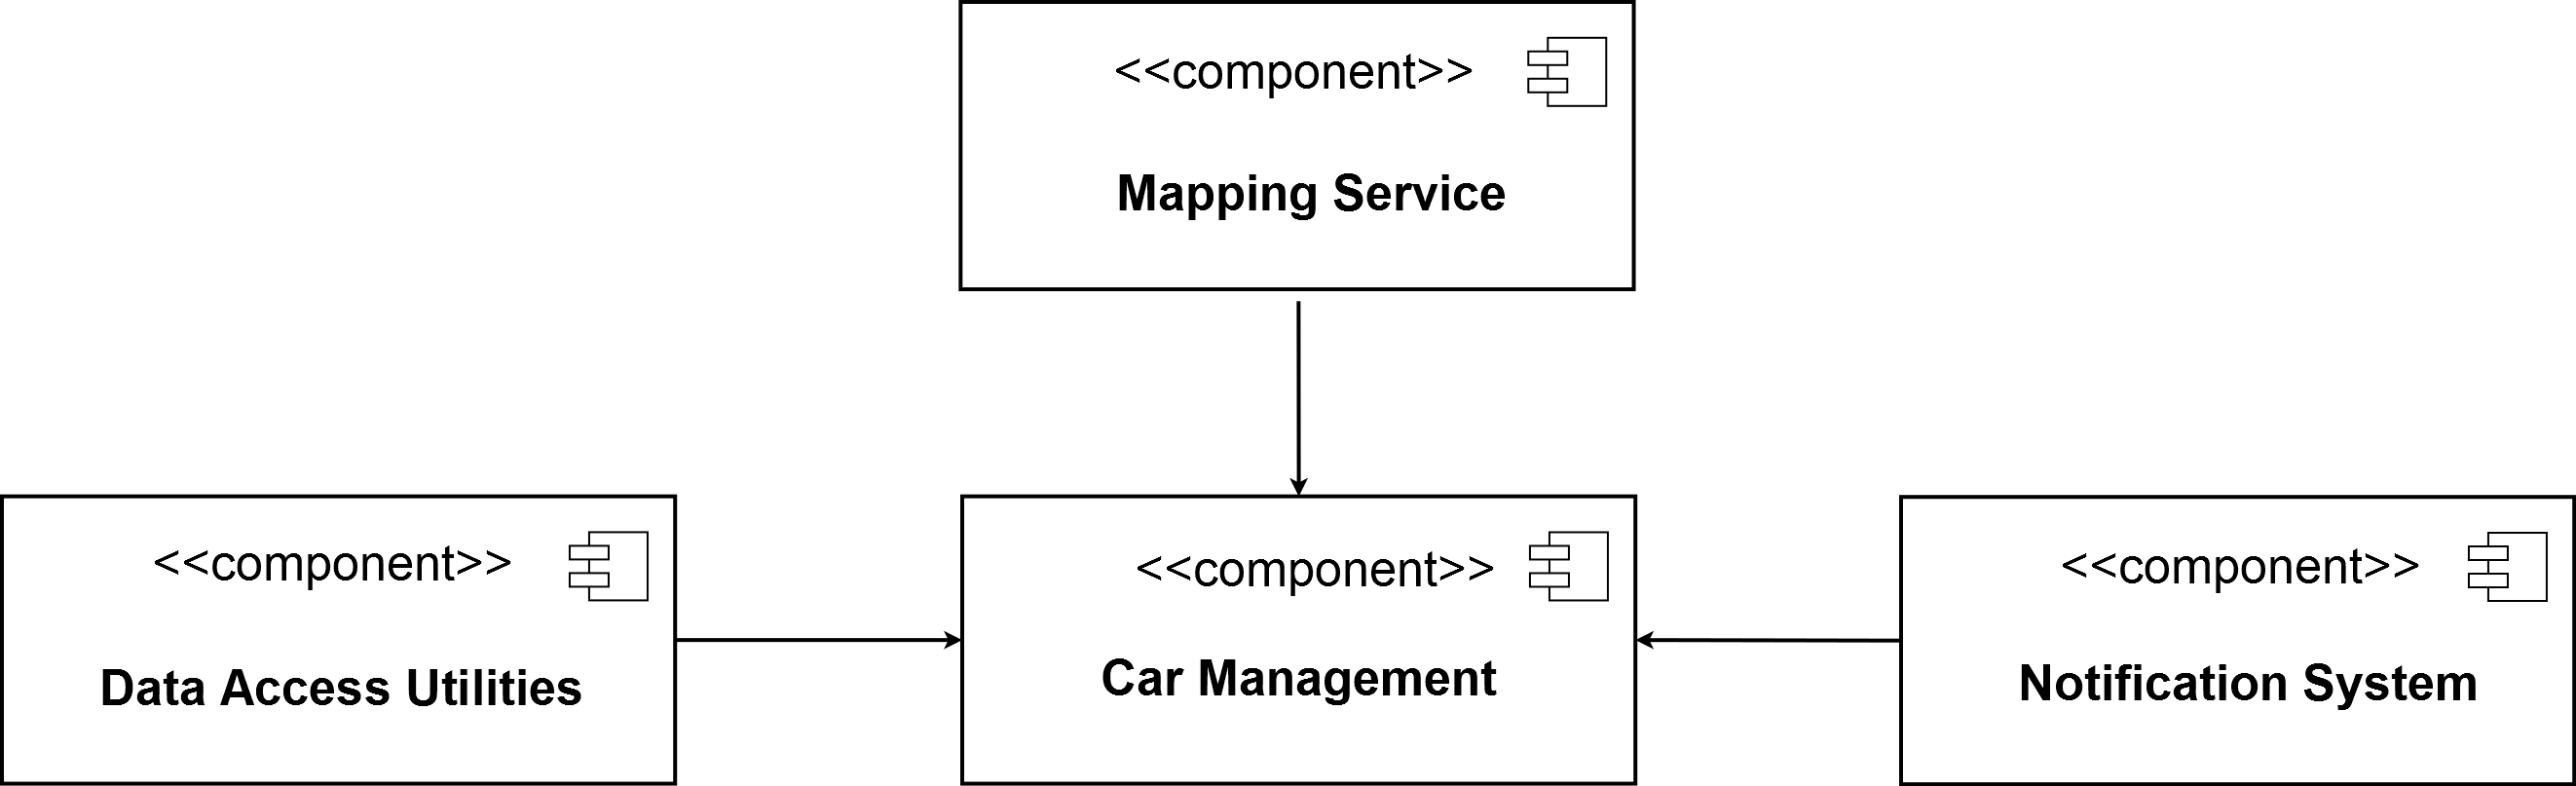
\includegraphics[scale=0.15]{Diagramma11}
   
  
  \newpage
  Now we are ready to integrate together the Reservation Management, Ride Management, Location Management and Car Management together in order to build the Car sharing subsystem:\\
   \vspace{1cm}
  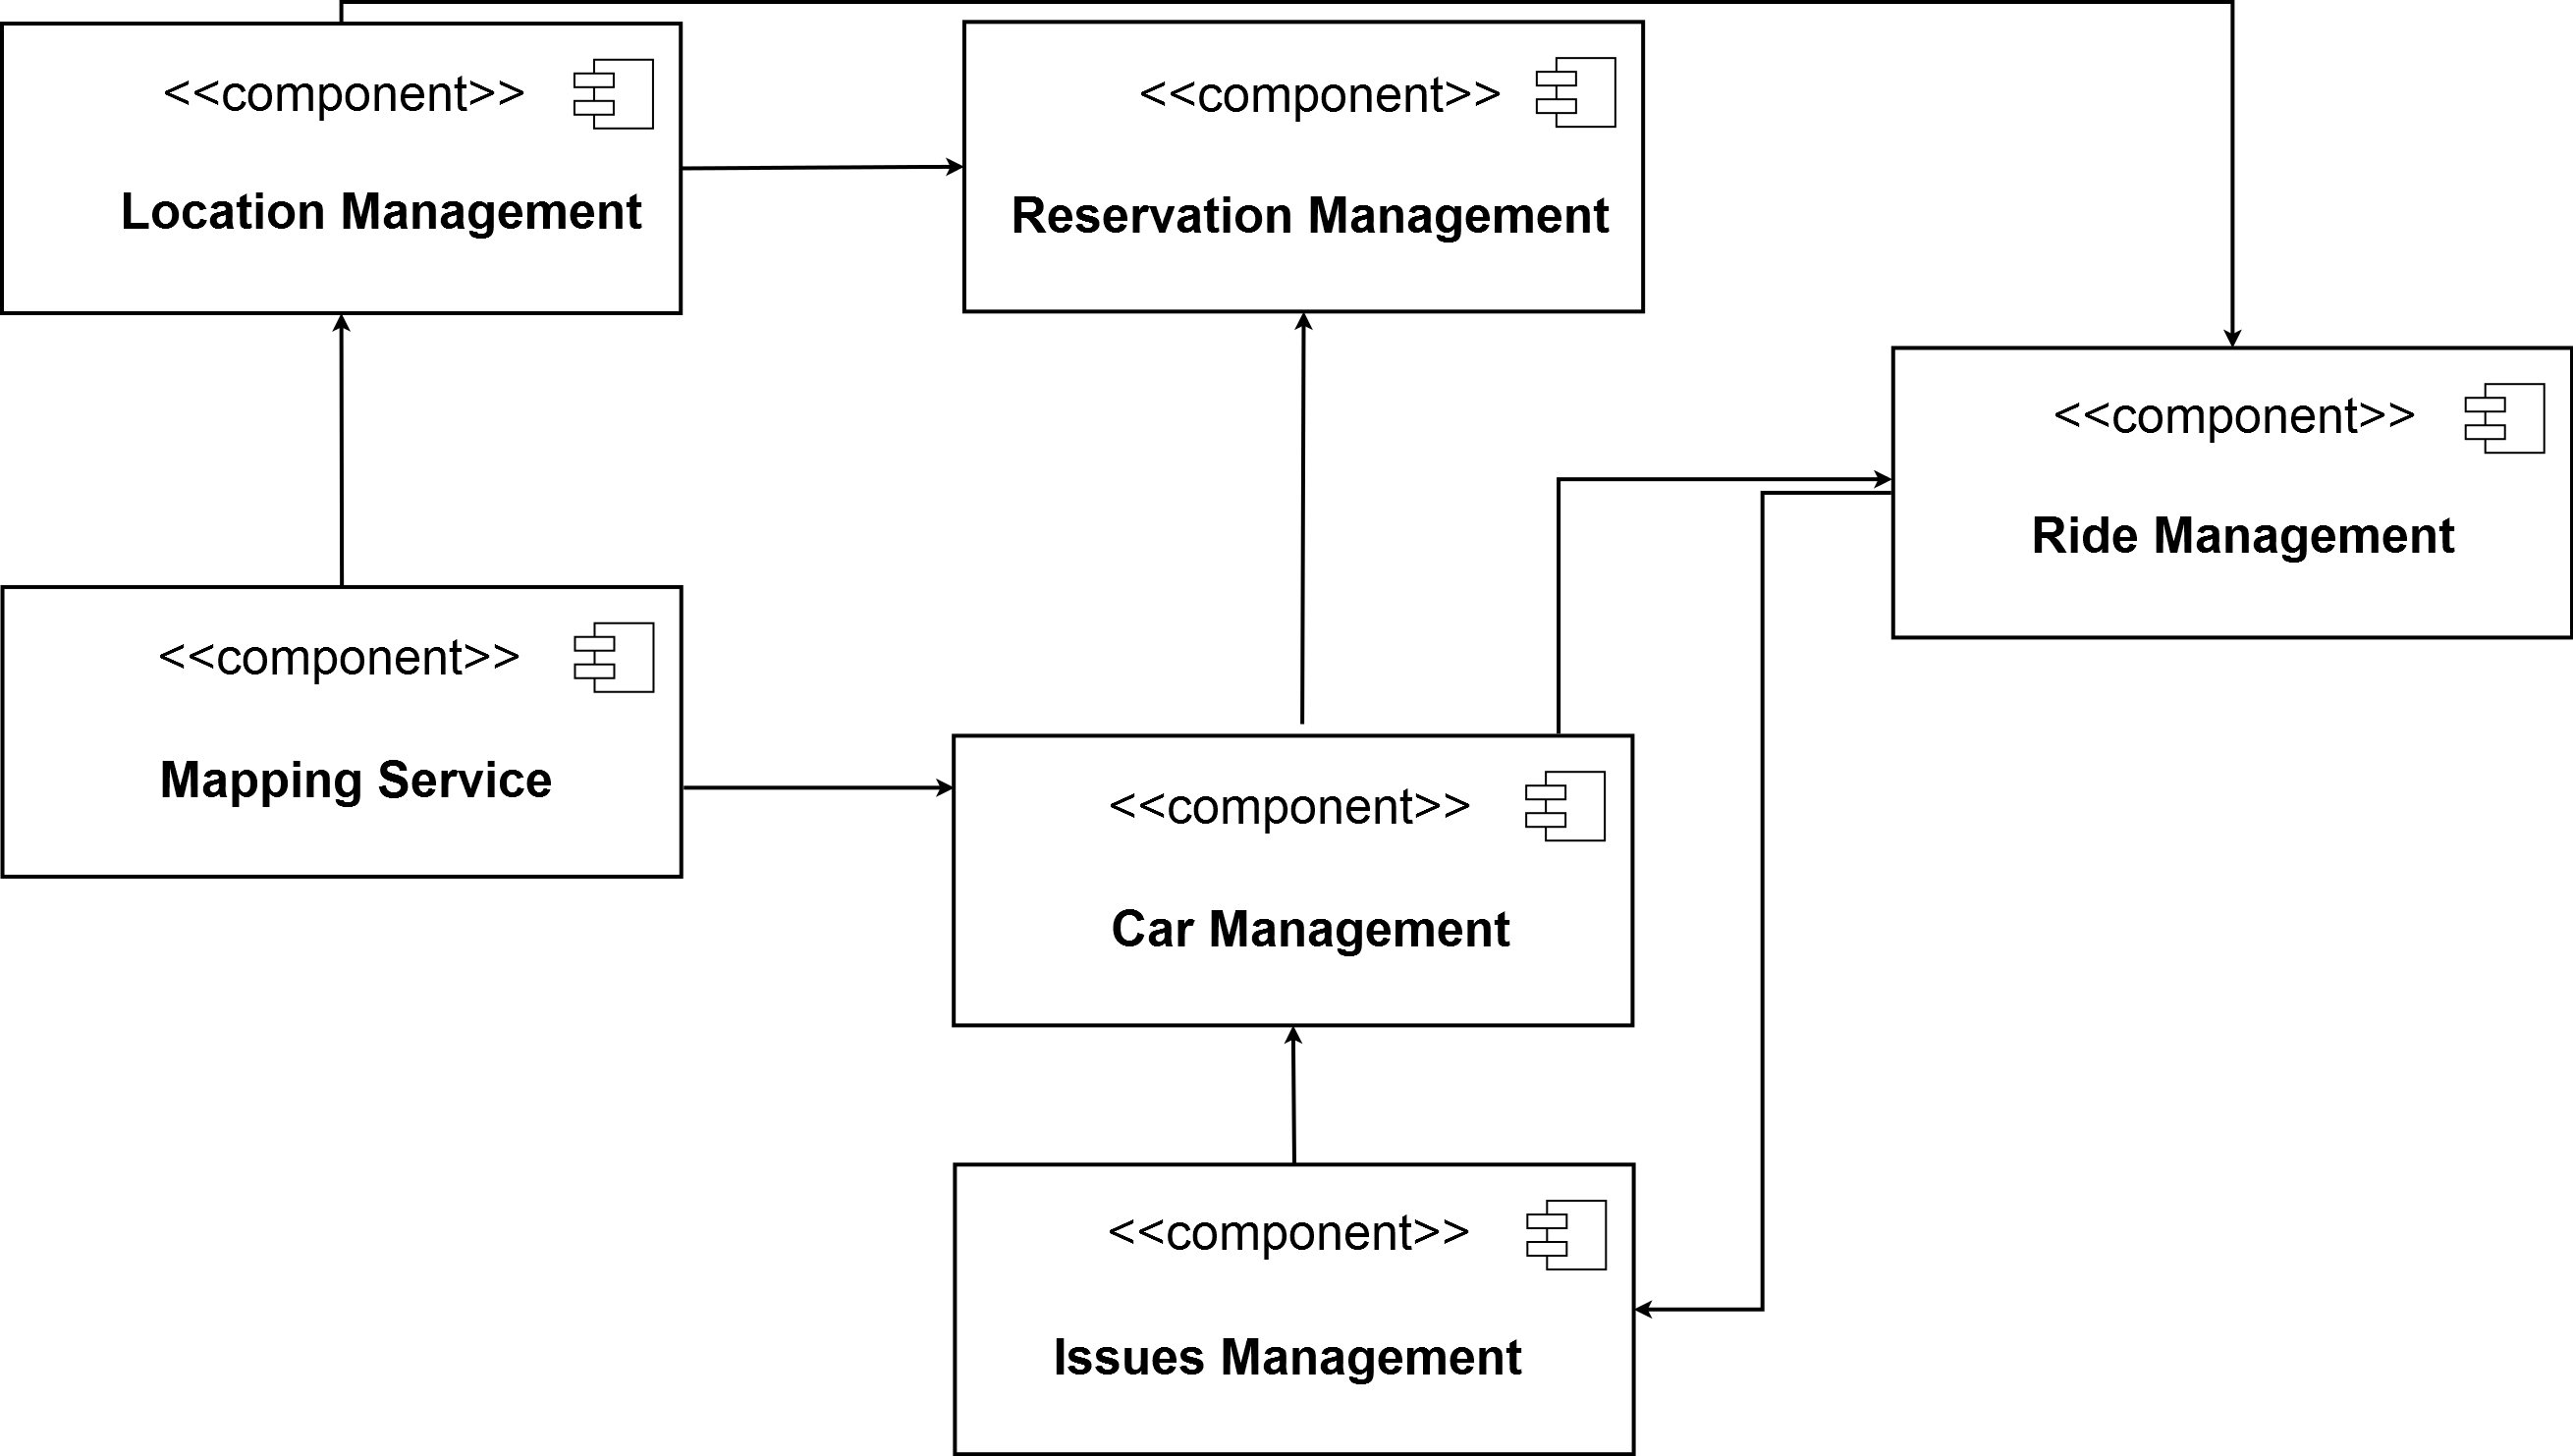
\includegraphics[scale=0.15]{Diagramma5}
 \newpage
    
  \textbf{System Administration} \\
  Following the critical-first strategy, the next step is to integrate the System Administration, which takes care of many important functions of the system ,  with the Notification System and the Data Access utilities. The System Administration is just a collection of subcomponents which are loosely correlated to each other, so they can be integrated with the rest of the system one by one in any order. The System Administration is just a wrapper for the methods of all its subcomponents. The way the components are integrated is showed below:\\
   \vspace{1cm}
  
  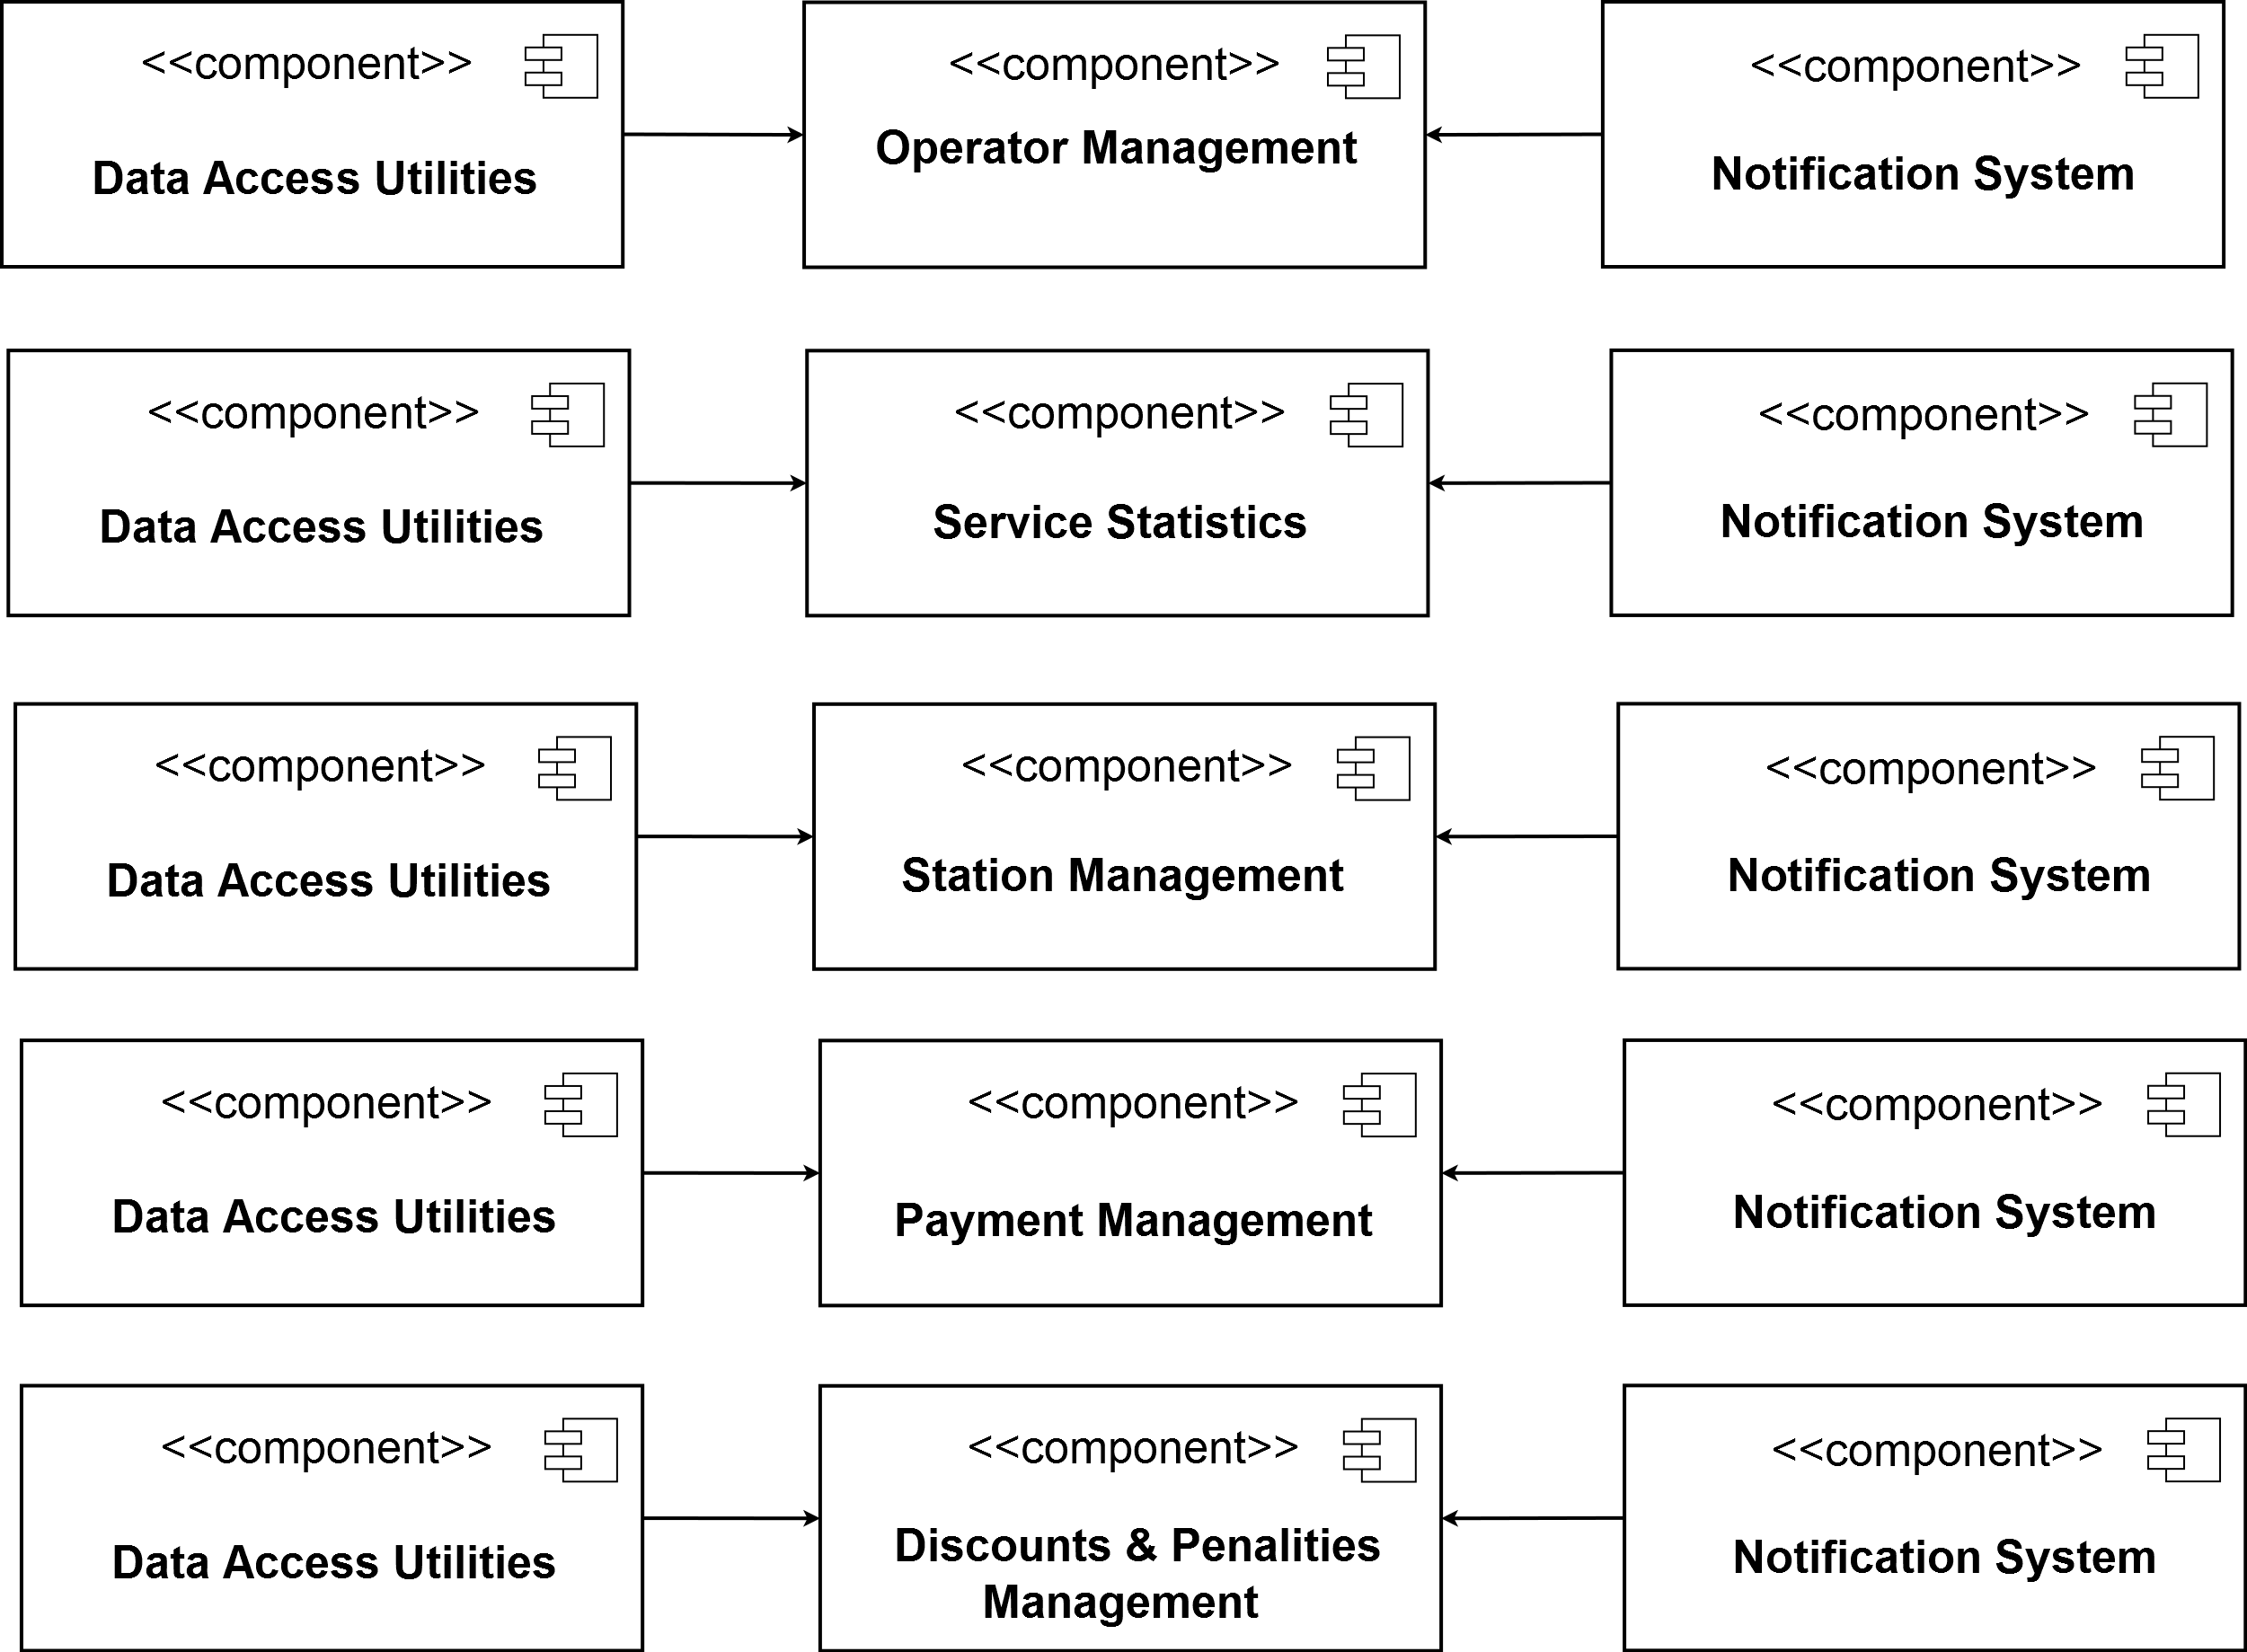
\includegraphics[scale=0.15]{Diagramma6}
  \newpage
  
  
  
  \textbf{Account Management} \\
  
  The next step consists in integrating the subcomponents of the Account Management subsystem. The subcomponents implementing this subsystem are not dependent from each other, thus they can be integrated independently with the rest of the system, in particular with the Notification system and the Data Access utilities.  Since these components are not really related to each other (each one of them takes care of a particular function related to the account management), the Account  Management subsystem is just a wrapper for their methods (just like the System Administration). The way the components are integrated is showed below:\\
  
  
  
   \vspace{1cm}
  
  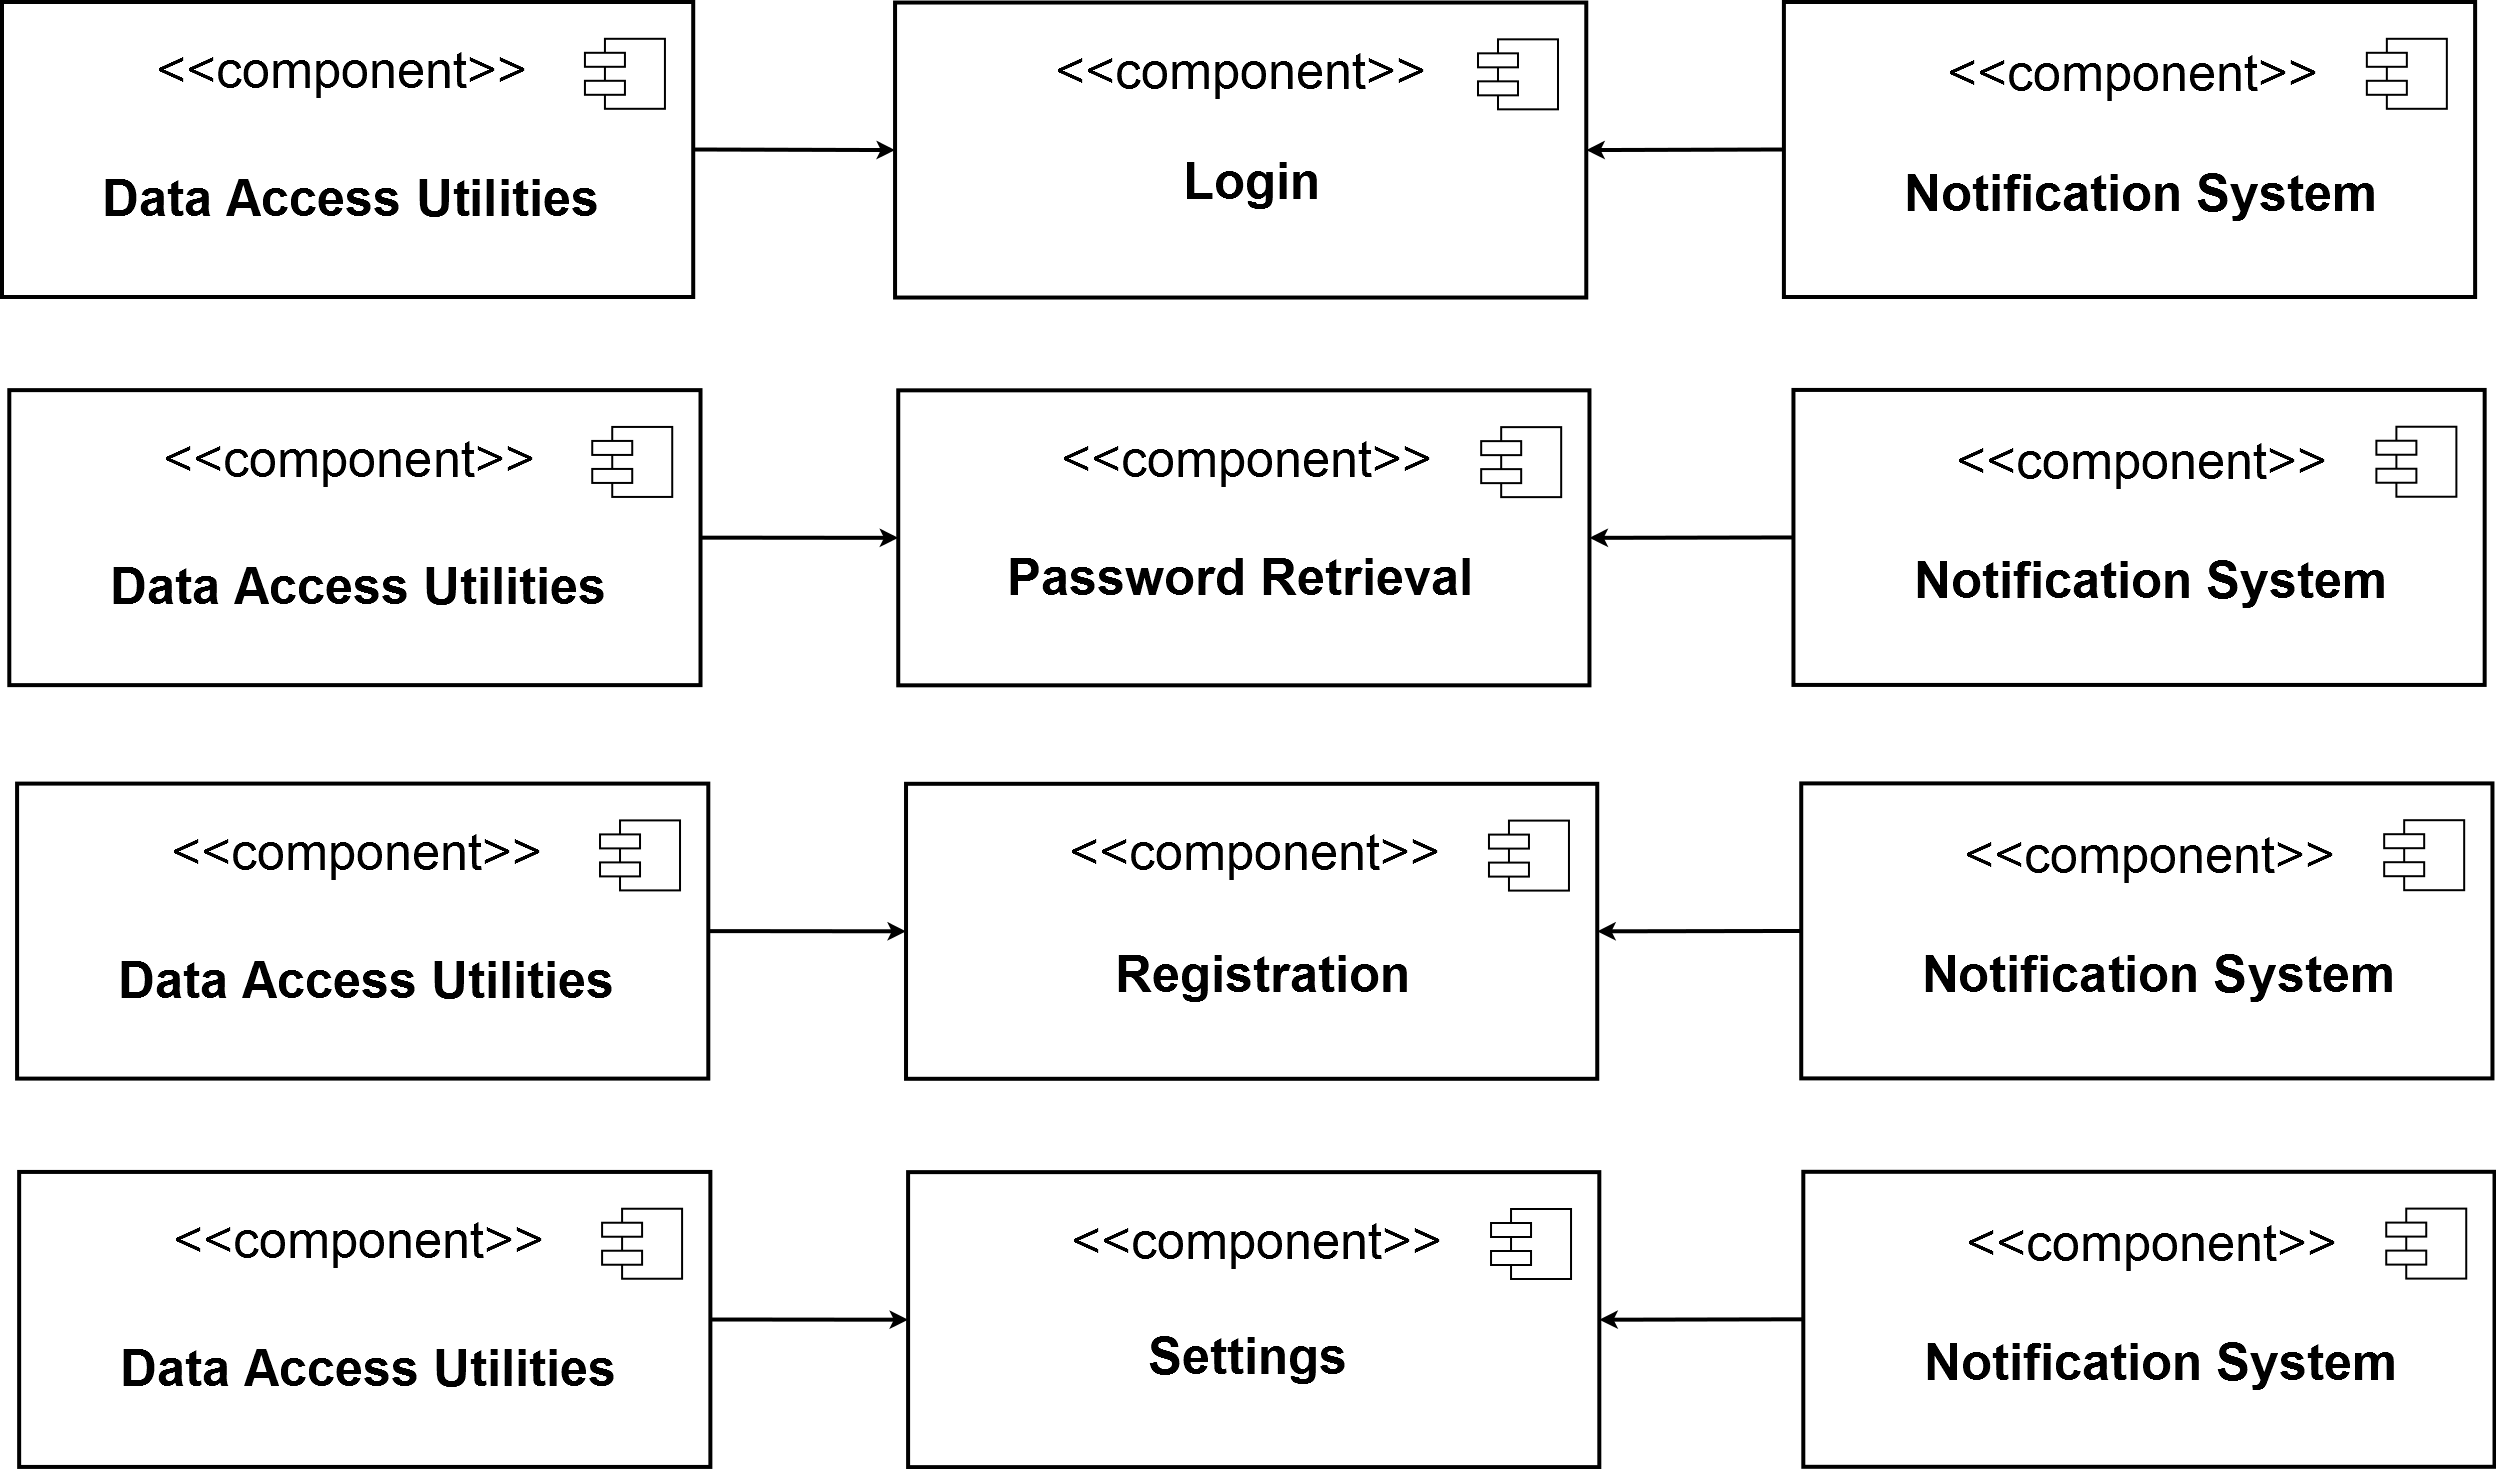
\includegraphics[scale=0.15]{Diagramma7}
  
  \newpage
   \subsubsection{Subsystem  Integration  Sequence}		% 2.4.2)SUBSYSTEM INTEGRATION SEQUENCE
   In the following diagram we provide a  detailed view of how the various high-level subsystems we build up to now have to be integrated together to create the full Power\&Joy system.\\
    \vspace{1cm}
     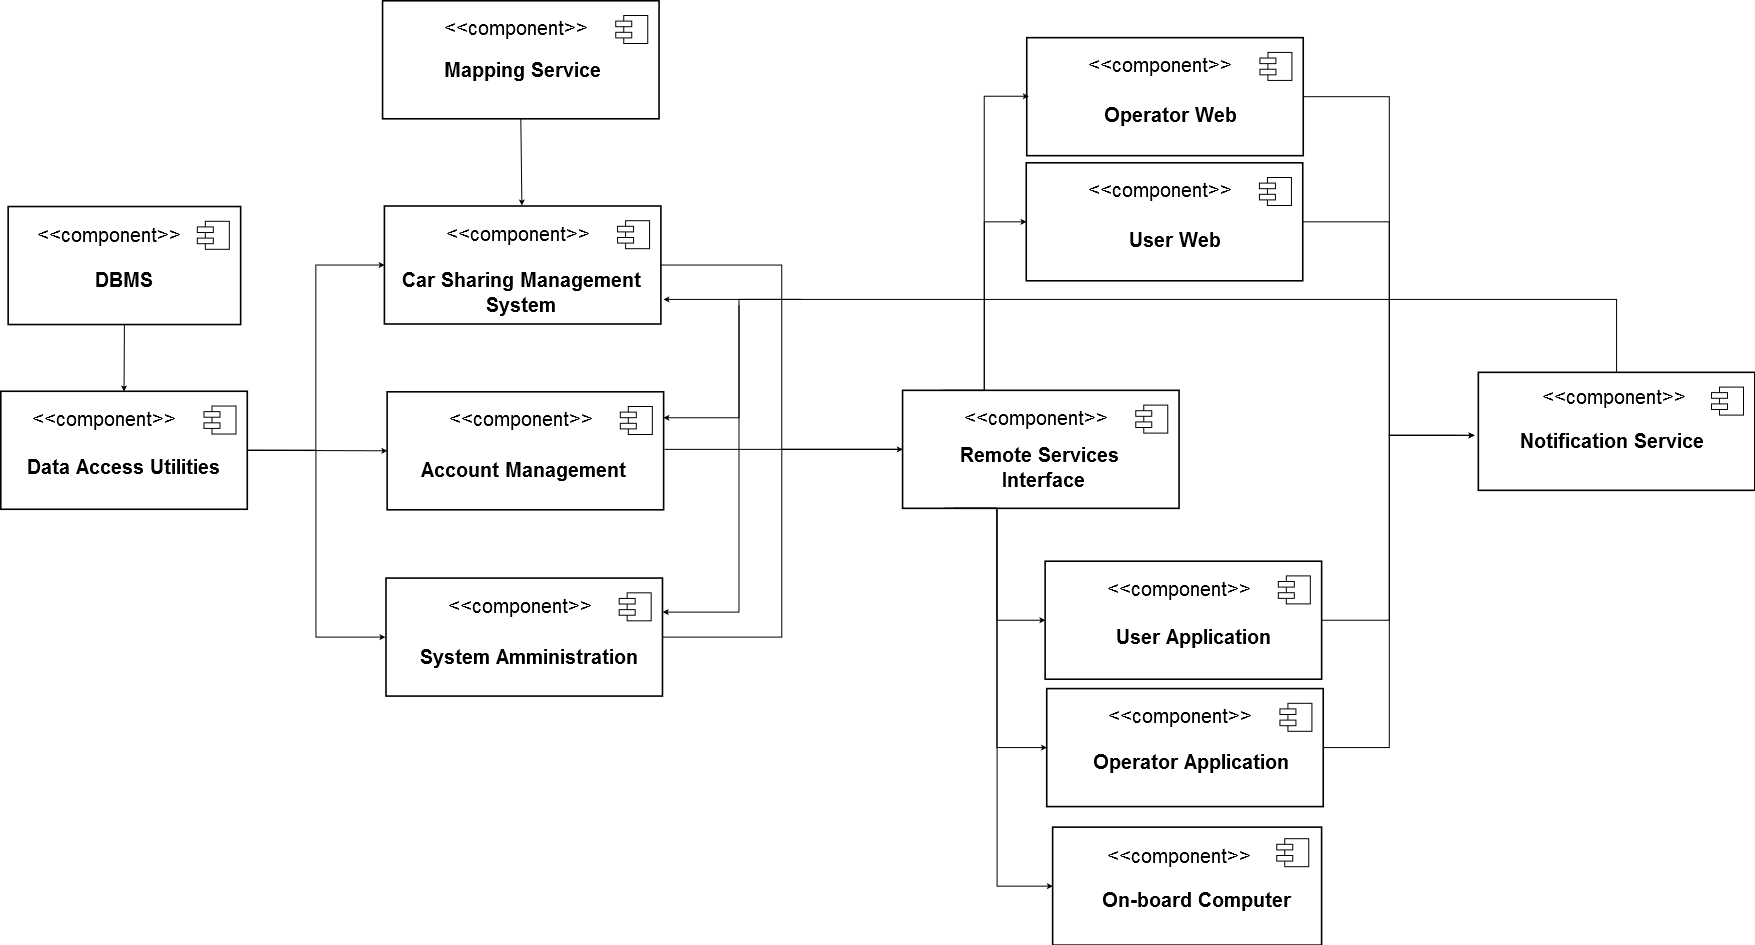
\includegraphics[scale=0.25]{Diagramma8}
     
     \newpage
  
  
  \section{Individual Steps and Test Description} 		% 3)INDIVIDUAL STEPS AND TEST DESCRIPTION
  
  \subsection{Car sharing management subsystem} %3.1)
  \subsubsection{Reservation Management, Data Access Utilities} %3.1.1)

     %TAB1
     \begin{center} 
    \begin {flushleft}
    \textbf{insertReservation(reservation)}
    \end{flushleft}
        \begin{tabular}{  |  p{6cm} | p{6cm} |}
    \hline
    \textit{input} &  \textit{effect} \\
    \hline
    
   Null parameter & NullArgumentException 
     \\ 
  \hline
  Reservation with an Id already existent in the database & InvalidArgumentValueException \\
  \hline
  Valid Argument & A tuple containing reservation data is inserted into the database \\
  \hline
    \end{tabular}
\end{center}

%TAB 2
\begin{center}
   \begin {flushleft}
    \textbf{deleteReservation(reservation)}
    \end{flushleft}
        \begin{tabular}{  |  p{6cm} | p{6cm} |}
    \hline
    \textit{input} &  \textit{effect} \\
    \hline
    
   Null Parameter &  NullArgumentException
     \\ 
  \hline
   reservation with an inexistent id &  nvalidArgumentValueException\\
  \hline
 Valid Argument &  The tuple containing reservation data is deleted from the database  \\
  \hline
    \end{tabular}
\end{center}

%  TAB 3
\begin{center}
   \begin {flushleft}
    \textbf{getReservationList()}
    \end{flushleft}
        \begin{tabular}{  |  p{6cm} | p{6cm} |}
    \hline
    \textit{input} &  \textit{effect} \\
    \hline
    
    Nothing &  The list of all the reservation on going \\

  
  \hline
    \end{tabular}
\end{center}


  
   \subsubsection{Ride Management, Data Access Utilities} %3.1.2)
   %TAB1
   
  \begin{center}
   \begin {flushleft}
    \textbf{endRide(ride)}
    \end{flushleft}
        \begin{tabular}{  |  p{6cm} | p{6cm} |}
    \hline
    \textit{input} &  \textit{effect} \\
    \hline
    
    Null Parameter & NullArgumentException 
     \\ 
  \hline
   RideId not found into the database & InvalidArgumentValueException  \\
  \hline
  Valid Argument & the tuple in the rideList is deleted     \\
  \hline
    \end{tabular}
\end{center}

%TAB2
\begin{center}
   \begin {flushleft}
    \textbf{insertRide(ride)}
    \end{flushleft}
        \begin{tabular}{  |  p{6cm} | p{6cm} |}
    \hline
    \textit{input} &  \textit{effect} \\
    \hline
    
   Null parameter & NullArgumentException 
     \\ 
  \hline
  Array with NULL fields & InvalidArgumentValueException  \\
  \hline
  Array with empty fields & InvalidArgumentValueException    \\
  \hline
  All the parameters inside ride tuple are valid & Entry is inserted inserted  into the database \\
  \hline
    \end{tabular}
\end{center}

 
 %TAB3
  \begin{center}
   \begin {flushleft}
    \textbf{getRideList()}
    \end{flushleft}
        \begin{tabular}{  |  p{6cm} | p{6cm} |}
    \hline
    \textit{input} &  \textit{effect} \\
    \hline
    
  Nothing & Returns a list with all the on-going rides
     \\ 
  
  \hline
    \end{tabular}
\end{center}

\newpage

%TAB4 
  \begin{center}
   \begin {flushleft}
    \textbf{getPassengers(ride)}
    \end{flushleft}
        \begin{tabular}{  |  p{6cm} | p{6cm} |}
    \hline
    \textit{input} &  \textit{effect} \\
    \hline
    
    Null parameter & NullArgumentException
     \\ 
  \hline
   The rideId is not found in the database &  InvalidArgumentValueException\\
  \hline
  Valid Argument & Returns the number of passengers inside the car when the ride ends    \\
  \hline
    \end{tabular}
\end{center}
   
   
   
    \subsubsection{Issue Management, Data Access Utilities}  %3.1.3)
    
    %TAB1
      \begin{center}
   \begin {flushleft}
    \textbf{getCarStatus(carId)}
    \end{flushleft}
        \begin{tabular}{  |  p{6cm} | p{6cm} |}
    \hline
    \textit{input} &  \textit{effect} \\
    \hline
    
    Null parameter & NullArgumentException
     \\ 
  \hline
   The carId is not found in the database & InvalidArgumentValueException  \\
  \hline
  The carId parameter is valid &  Returns the status of the car corresponding to the Id inserted  \\
  \hline
    \end{tabular}
\end{center}


%TAB2
  \begin{center}
   \begin {flushleft}
    \textbf{getAccidentCarList()}
    \end{flushleft}
        \begin{tabular}{  |  p{6cm} | p{6cm} |}
    \hline
    \textit{input} &  \textit{effect} \\
    \hline
    
    Nothing & Returns a list with all the cars implicated in an accident 
     \\ 

  \hline
    \end{tabular}
\end{center}

%TAB3
  \begin{center}
   \begin {flushleft}
    \textbf{getLowChargeCarList()}
    \end{flushleft}
        \begin{tabular}{  |  p{6cm} | p{6cm} |}
    \hline
    \textit{input} &  \textit{effect} \\
    \hline
    
    Nothing & Returns a list with all the cars with no more than 20\% of battery charge 
     \\ 

  \hline
    \end{tabular}
\end{center}

%TAB4
  \begin{center}
   \begin {flushleft}
    \textbf{getAssistanceNeededCarList()}
    \end{flushleft}
        \begin{tabular}{  |  p{6cm} | p{6cm} |}
    \hline
    \textit{input} &  \textit{effect} \\
    \hline
    
    Nothing & Returns a list with all the cars that need assistance. It differs from accident because ?assistance needed? status is marked when an user find issues inside/outside the car when he reserve it 
     \\ 

  \hline
    \end{tabular}
\end{center}

%TAB5
  \begin{center}
   \begin {flushleft}
    \textbf{getIssuedCarList()}
    \end{flushleft}
        \begin{tabular}{  |  p{6cm} | p{6cm} |}
    \hline
    \textit{input} &  \textit{effect} \\
    \hline
    
    Nothing & Returns a list with all the cars and their status
     \\ 

  \hline
    \end{tabular}
\end{center}
    
    \newpage
    
     \subsubsection{Car Management, Data Access Utilities} %3.1.4)
     
     %TAB1
       \begin{center}
   \begin {flushleft}
    \textbf{changeCarStatus(carId, newStatus)}
    \end{flushleft}
        \begin{tabular}{  |  p{6cm} | p{6cm} |}
    \hline
    \textit{input} &  \textit{effect} \\
    \hline
    
    Null parameter & NullArgumentException 
     \\ 
  \hline
   nvalid Status (the possible status are noIssues, LowCharge, Accident, AssistanceNeeded) & InvalidArgumentValueException \\
  \hline
  The new status is equal to the previous one &  Status of the car does not change  \\
  \hline
  Valid Argument & The status of the car is updated with  new entry\\
  \hline

    \end{tabular}
\end{center}

%TAB2
  \begin{center}
   \begin {flushleft}
    \textbf{getBatteryCharge(carId)}
    \end{flushleft}
        \begin{tabular}{  |  p{6cm} | p{6cm} |}
    \hline
    \textit{input} &  \textit{effect} \\
    \hline
    
    Null parameter & NullArgumentException
     \\ 
  \hline
   The carId does not exist in the database &  InvalidArgumentValueException \\
  \hline
  Valid Argument & Returns the percentage of the battery    \\
  \hline
    \end{tabular}
\end{center}

%TAB3
  \begin{center}
   \begin {flushleft}
    \textbf{insertCar(carId)}
    \end{flushleft}
        \begin{tabular}{  |  p{6cm} | p{6cm} |}
    \hline
    \textit{input} &  \textit{effect} \\
  
  \hline
   Null parameter & NullArgumentException \\
  \hline
  Valid Argument &  The car is uploaded into the database  \\
  \hline
    \end{tabular}
\end{center}

%TAB4
  \begin{center}
   \begin {flushleft}
    \textbf{deleteCar(carId)}
    \end{flushleft}
        \begin{tabular}{  |  p{6cm} | p{6cm} |}
    \hline
    \textit{input} &  \textit{effect} \\
  
  \hline
   Null parameter & NullArgumentException \\
  \hline
  Valid Argument & The car is deleted from the database    \\
  \hline
    \end{tabular}
\end{center}

%TAB5
  \begin{center}
   \begin {flushleft}
    \textbf{isAvailableCar(carId)}
    \end{flushleft}
        \begin{tabular}{  |  p{6cm} | p{6cm} |}
    \hline
    \textit{input} &  \textit{effect} \\
    \hline
    
    Null parameter & NullArgumentException
     \\ 
  \hline
   A car with an id inexistent into the database & InvalidArgumentValueException  \\
  \hline
  Car available & returns true    \\
  \hline
  
  Car unavailable & returns false \\
  \hline
    \end{tabular}
\end{center}


%TAB6
  \begin{center}
   \begin {flushleft}
    \textbf{getAvailableCarList()}
    \end{flushleft}
        \begin{tabular}{  |  p{6cm} | p{6cm} |}
    \hline
    \textit{input} &  \textit{effect} \\
    \hline
    
    Nothing & Returns the list of all the car available when the method is called 
     \\ 

  \hline
    \end{tabular}
\end{center}

%TAB 7
  \begin{center}
   \begin {flushleft}
    \textbf{reportLowCharger(carId, userId)}
    \end{flushleft}
        \begin{tabular}{  |  p{6cm} | p{6cm} |}
    \hline
    \textit{input} &  \textit{effect} \\
    \hline
    
    Null parameter & NullArgumentException
     \\ 
  \hline
Valid Paramters & In the end of the ride the method ?changeStatusCar? is called with LowCharge as parameter\\
  \hline

    \end{tabular}
\end{center}
     
\subsubsection{Reservation  Management, Issues Management}%3.1.5)

%TAB1

  \begin{center}
   \begin {flushleft}
    \textbf{reportAssistanceNeeded(carId, userId)}
    \end{flushleft}
        \begin{tabular}{  |  p{6cm} | p{6cm} |}
    \hline
    \textit{input} &  \textit{effect} \\
    \hline
    
   Null parameter & NullArgumentException 
    
     \\ 
  \hline
   Valid Parameters & The user reports a problem inside/outside the car and the system calls the method ?changeStatusCar? with ?assistanceNeeded? as parameter  \\
  \hline

    \end{tabular}
\end{center}




%INSERIRE REPORT VARI
     
      \subsubsection{Car Manegement, Location Management } %3.1.6)
      
      %TAB1
        \begin{center}
   \begin {flushleft}
    \textbf{isSafeArea(position)}
    \end{flushleft}
        \begin{tabular}{  |  p{6cm} | p{6cm} |}
    \hline
    \textit{input} &  \textit{effect} \\
    \hline
    
    Null parameter & NullArgumentException
     \\ 
  \hline
   A position whose coordinates are invalid & InvalidArgumentValueException \\
  \hline
  A position outside the safe area & Returns false    \\
  \hline
  A position inside the safe area & Returns True \\
  \hline
    \end{tabular}
\end{center}

%TAB2
  \begin{center}
   \begin {flushleft}
    \textbf{getPosition(carId)}
    \end{flushleft}
        \begin{tabular}{  |  p{6cm} | p{6cm} |}
    \hline
    \textit{input} &  \textit{effect} \\
    \hline
    
    Null parameter & NullArgumentException
     \\ 
  \hline
   The carId is not found in the database & InvalidArgumentValueException \\
  \hline
  CarId exist in the database & Return the current position of the car
   \\
  \hline
    \end{tabular}
\end{center}
      
      
      
      \subsubsection{Reservation Manegement, Location Management } %3.1.7
      
        \begin{center}
   \begin {flushleft}
    \textbf{getPosition()}
    \end{flushleft}
        \begin{tabular}{  |  p{6cm} | p{6cm} |}
    \hline
    \textit{input} &  \textit{effect} \\
    \hline
    
    Null parameter & NullArgumentException
     \\ 
  \hline
  Valid Parameter & Return the current position of the car  \\
  \hline

    \end{tabular}
\end{center}
      
      \subsubsection{Ride Management, Location Management} %3.1.8
             \begin{center}
   \begin {flushleft}
    \textbf{getPosition()}
    \end{flushleft}
        \begin{tabular}{  |  p{6cm} | p{6cm} |}
    \hline
    \textit{input} &  \textit{effect} \\
    \hline
    
    Null parameter & NullArgumentException
     \\ 
  \hline
  Valid Parameter & Return the current position of the car  \\
  \hline

    \end{tabular}
\end{center} 
      
     \newpage 
       \subsubsection{Reservation Management, Car Management} %3.1.9
       
   \begin{center}    
          \begin {flushleft}
    \textbf{unlockReservedCar(userId)}
    \end{flushleft}
        \begin{tabular}{  |  p{6cm} | p{6cm} |}
    \hline
    \textit{input} &  \textit{effect} \\
    \hline
    
    Null parameter & NullArgumentException 
     \\ 
  \hline
   The userId (contactless card) and the Id of the user that reserve the car are not the same & InvalidArgumentValueException, the system do not unlock the doors \\
  \hline
  The userId (contactless card) and the Id of the user that reserve the car match&  The system unlocks the doors of the car \\
  \hline
    \end{tabular}
\end{center}
       
       
         \subsubsection{Ride Management, Issues Management}
         
          
           \begin{center}
   \begin {flushleft}
    \textbf{reportAccident(carId, userId)}
    \end{flushleft}
        \begin{tabular}{  |  p{6cm} | p{6cm} |}
    \hline
    \textit{input} &  \textit{effect} \\
    \hline
    
    Null parameter & NullArgumentException
     \\ 
  \hline
  Valid Parameters &  The user reports the accident and the system calls the method ?changeStatusCar? with ?Accident? as parameter to mark car as unavailable \\
  \hline

    \end{tabular}
\end{center} 
           
           
       
      
   \subsection{Administration subsystem} %3.2
    \subsubsection{Operator Management, Data Access Utilities}
    
       
  \begin{center}
   \begin {flushleft}
    \textbf{insertOperator(operatorId)}
    \end{flushleft}
        \begin{tabular}{  |  p{6cm} | p{6cm} |}
    \hline
    \textit{input} &  \textit{effect} \\
    \hline
    
      Null parameter & NullArgumentException
     \\ 
  \hline
   Valid Parameter &   The operator data is inserted into the database\\
  \hline

    \end{tabular}
\end{center}


   
  \begin{center}
   \begin {flushleft}
    \textbf{deleteOperator(operatorId)}
    \end{flushleft}
        \begin{tabular}{  |  p{6cm} | p{6cm} |}
    \hline
    \textit{input} &  \textit{effect} \\
    \hline
    
      Null parameter & NullArgumentException
     \\ 
  \hline
   alid Parameter &  The operator data is deleted from the database\\
  \hline

    \end{tabular}
\end{center}


   
  \begin{center}
   \begin {flushleft}
    \textbf{operate(carId)}
    \end{flushleft}
        \begin{tabular}{  |  p{6cm} | p{6cm} |}
    \hline
    \textit{input} &  \textit{effect} \\
    \hline
    
    Null parameter & NullArgumentException
     \\ 
  \hline
   The parameter has as  car status ''noIssues'' &  InvalidArgumentValueException \\
  \hline
Valid argument, the car has at least one issue  &  The system marks that car as unavailable and the operator have to resolve the issue(s) on that car. The system adds the car to the list of cars that are being repaired  \\
  \hline
    \end{tabular}
\end{center}


   
  \begin{center}
   \begin {flushleft}
    \textbf{IssueSolved(carId)}
    \end{flushleft}
        \begin{tabular}{  |  p{6cm} | p{6cm} |}
    \hline
    \textit{input} &  \textit{effect} \\
    \hline
    
    Null parameter & NullArgumentException
     \\ 
  \hline
   The car is not present inside the list of the car that are being repaired &  InvalidArgumentValueException\\
  \hline
 Valid Argument & The car is repaired, its status get back to ?noIssues? and it is available to be reserved again    \\
  \hline
    \end{tabular}
\end{center}




   
  \begin{center}
   \begin {flushleft}
    \textbf{getoperatorList()}
    \end{flushleft}
        \begin{tabular}{  |  p{6cm} | p{6cm} |}
    \hline
    \textit{input} &  \textit{effect} \\
    \hline
    
    Nothing & The list of all operators in the database
     \\ 
  \hline
 
    \end{tabular}
\end{center}



   
  \begin{center}
   \begin {flushleft}
    \textbf{getStation(operator)}
    \end{flushleft}
        \begin{tabular}{  |  p{6cm} | p{6cm} |}
    \hline
    \textit{input} &  \textit{effect} \\
    \hline
    
    Null parameter & NullArgumentException
     \\ 
  \hline
   Valid Argument & Returns the name of the station where the operator actually works \\
  \hline
 
    \end{tabular}
\end{center}
    
    
    
    
     
     
     
     
     
     
      \subsubsection{Station Management, Data Access Utilities}
      
      
        \begin{center}
   \begin {flushleft}
    \textbf{getStationPosition(stationId)}
    \end{flushleft}
        \begin{tabular}{  |  p{6cm} | p{6cm} |}
    \hline
    \textit{input} &  \textit{effect} \\
    \hline
    
    Null parameter & NullArgumentException
     \\ 
  \hline
  The Station is not found in the database & InvalidArgumentValueException \\
  \hline
  The station is found in the database &  Returns the position of the station
  \\
  \hline
    \end{tabular}
\end{center}


  \begin{center}
   \begin {flushleft}
    \textbf{getOperatorsList(stationId)}
    \end{flushleft}
        \begin{tabular}{  |  p{6cm} | p{6cm} |}
    \hline
    \textit{input} &  \textit{effect} \\
    \hline
    
    Null parameter & NullArgumentException
     \\ 
  \hline
   The Station is not found in the database & InvalidArgumentValueException  \\
  \hline
  The station is found in the database& Returns a list of all the operators that work in that station   \\
  \hline
    \end{tabular}
\end{center}


  \begin{center}
   \begin {flushleft}
    \textbf{insertStation(station)}
    \end{flushleft}
        \begin{tabular}{  |  p{6cm} | p{6cm} |}
    \hline
    \textit{input} &  \textit{effect} \\
    \hline
    
     Null parameter & NullArgumentException
     \\ 
  \hline
   Invalid or null arguments or the station already exists in the database &  InvalidArgumentValueException \\
  \hline
  valid argument & The station data are uploaded into the database    \\
  \hline
    \end{tabular}
\end{center}

\newpage

  \begin{center}
   \begin {flushleft}
    \textbf{deleteStation()}
    \end{flushleft}
        \begin{tabular}{  |  p{6cm} | p{6cm} |}
    \hline
    \textit{input} &  \textit{effect} \\
    \hline
    
    Null parameter & NullArgumentException
     \\ 
  \hline
  The station is not found in the database &  InvalidArgumentValueException  \\
  \hline
  The station is found in the database & The station data of that station are deleted
   \\
  \hline
    \end{tabular}
\end{center}
      
      
      
      
      
      
    
      
      
      
       \subsubsection{Payment Management, Data Access Utilities}
       
       
       \begin{center}
   \begin {flushleft}
    \textbf{SendRidePaymentInformation(price, creditCardNumber)}
    \end{flushleft}
        \begin{tabular}{  |  p{6cm} | p{6cm} |}
    \hline
    \textit{input} &  \textit{effect} \\
    \hline
    
    Null parameter & NullArgumentException 
     \\ 
  \hline
  Price is negative & InvalidArgumentValueException   \\
  \hline
 Valid Argument &  All the information are sent to the Payment System in order  to pay the ride   \\
  \hline
    \end{tabular}
\end{center}
       
       
       
       
       
        \subsubsection{Discounts\&Penalities Management, Data Access Utilities}
        
        
        \begin{center}
   \begin {flushleft}
    \textbf{apply(percentage)}
    \end{flushleft}
        \begin{tabular}{  |  p{6cm} | p{6cm} |}
    \hline
    \textit{input} &  \textit{effect} \\
    \hline
    
      Null parameter & NullArgumentException
     \\ 
  \hline
   Valid Argument & The ride cost is modified adding the percentage of  the ride  \\
 
  \hline
    \end{tabular}
\end{center}
        
        
 
        
        
   \newpage     
    \subsection{Account Management subsystem} %3.3
     \subsubsection{Login Management, Data Access Utilities}
     
       \begin{center}
   \begin {flushleft}
    \textbf{checkPassword(userId, password)}
    \end{flushleft}
        \begin{tabular}{  |  p{6cm} | p{6cm} |}
    \hline
    \textit{input} &  \textit{effect} \\
    \hline
    
    Null parameter & NullArgumentException 
     \\ 
  \hline
   userId is inexistent in the database & InvalidArgumentValueException \\
  \hline
  Not valid combination of userId and password &  InvalidCredentialsException  \\
  \hline
  Valid combination of parameters & Returns user home page \\
  \hline
    \end{tabular}
\end{center}
     
     
      \subsubsection{Password Retrieval, Data Access Utilities}
      
      
        \begin{center}
   \begin {flushleft}
    \textbf{forgotPassword(userid, email)}
    \end{flushleft}
        \begin{tabular}{  |  p{6cm} | p{6cm} |}
    \hline
    \textit{input} &  \textit{effect} \\
    \hline
    
    Null parameter & NullArgumentException 
     \\ 
  \hline
  userId is inexistent in the database & InvalidArgumentValueException \\
  \hline
  Not valid combination of userId and email &  InvalidCredentialsException   \\
  \hline
  Valid combination of parameters & An email is sent to the user in order to change his password\\
    \end{tabular}
\end{center}
      
      
       \subsubsection{Registration, Data Access Utilities }
       
         \begin{center}
   \begin {flushleft}
    \textbf{insertUser(user)}
    \end{flushleft}
        \begin{tabular}{  |  p{6cm} | p{6cm} |}
    \hline
    \textit{input} &  \textit{effect} \\
    \hline
    
    Null parameter & NullArgumentException
     \\ 
  \hline
   Valid user & The user data is inserted into the database \\
  \hline

    \end{tabular}
\end{center}


  \begin{center}
   \begin {flushleft}
    \textbf{deleteUser(userId)}
    \end{flushleft}
        \begin{tabular}{  |  p{6cm} | p{6cm} |}
    \hline
    \textit{input} &  \textit{effect} \\
    \hline
    
     Null parameter & NullArgumentException
     \\ 
  \hline
  Valid user &  The user data is deleted from the database
\\
  \hline
  

    \end{tabular}
\end{center}
       
       
       
        \subsubsection{Settings, Data Access Utilities}
          \begin{center}
   \begin {flushleft}
    \textbf{updateAccount(userId, userData)}
    \end{flushleft}
        \begin{tabular}{  |  p{6cm} | p{6cm} |}
    \hline
    \textit{input} &  \textit{effect} \\
    \hline
    
    Null parameter & NullArgumentException
     \\ 
  \hline
  UserId not found in the database or not Valid Data &  InvalidArgumentValueException   \\
  \hline
 Valid user and data &   The user data is updated in the database
 \\
  \hline
    \end{tabular}
\end{center}
    
    
    
        
     \subsection{Integration among subsystems} %3.4
     
     
     
      \subsubsection{Remote Services Interface, Car Sharing Subsystem}
      
      %FINIRE QUA
      
      
         \begin{center}
   \begin{flushleft}
    \textbf{reserveCar(carId, userId)}
    \end{flushleft}
        \begin{tabular}{  |  p{6cm} | p{6cm} |}
    \hline
    \textit{input} &  \textit{effect} \\
    \hline
    
    Null parameter & NullArgumentException
     \\ 
  \hline
   not valid  userId & InvalidArgumentValueException  \\
  \hline
   Not valid  carId & InvalidArgumentValueException  \\
  \hline
  Valid userId and  car & the system reserves the car for the user  \\
  \hline
    \end{tabular}
\end{center}


   \begin{center}
   \begin{flushleft}
    \textbf{startRide(userId, carId)}
    \end{flushleft}
        \begin{tabular}{  |  p{6cm} | p{6cm} |}
    \hline
    \textit{input} &  \textit{effect} \\
    \hline
    
    Null parameter & NullArgumentException
     \\ 
  \hline
   Not valid userId & InvalidArgumentValueException  \\
  \hline
   Not valid  carId & InvalidArgumentValueException  \\
  \hline
   Not valid  reservation associated to the user & InvalidArgumentValueException  \\
  \hline
  Valid user  and car identifiers, valid reservation &  the reservation is cancelled and a new ride is created   \\
  \hline
    \end{tabular}
\end{center}



   \begin{center}
   \begin{flushleft}
    \textbf{endRide(rideId)}
    \end{flushleft}
        \begin{tabular}{  |  p{6cm} | p{6cm} |}
    \hline
    \textit{input} &  \textit{effect} \\
    \hline
    
    Null parameter & NullArgumentException
     \\ 
  \hline
   Not valid rideId & InvalidArgumentValueException  \\
  \hline
  Valid rideId & The system  ends  the ride  \\
  \hline
    \end{tabular}
\end{center}
      
      
      
      
      
      
      
      
      
      
      
      
      
      
      
      
      
      
      
      
      
      
      
      
      
      
      
      
      
      
      
      
      
      
      
      
      
      
      
      \subsubsection{Remote Services Interface, Account Manager } %3.4.2
      
   \begin{center}
   \begin{flushleft}
    \textbf{insertUser(user)}
    \end{flushleft}
        \begin{tabular}{  |  p{6cm} | p{6cm} |}
    \hline
    \textit{input} &  \textit{effect} \\
    \hline
    
    Null parameter & NullArgumentException
     \\ 
  \hline
   not valid/ already existent user & InvalidArgumentValueException  \\
  \hline
  Valid user & The user data is inserted  into the database and the registration confirmation is sent to him    \\
  \hline
    \end{tabular}
\end{center}


  \begin{center}
   \begin {flushleft}
    \textbf{deleteUser(userId)}
    \end{flushleft}
        \begin{tabular}{  |  p{6cm} | p{6cm} |}
    \hline
    \textit{input} &  \textit{effect} \\
    \hline
    
    Null parameter & NullArgumentException
     \\ 
  \hline
  The userId does not exist in the database & InvalidArgumentValueException  \\
  \hline
  Th userId is found in the database & The user data is removed from the database
   \\
  \hline
    \end{tabular}
\end{center}
      
      
      
      
      
      
      
      \subsubsection{Remote Services Interface, Administration Subsystem}
      
   \begin{center}
   \begin {flushleft}
    \textbf{insertoperator(operator)}
    \end{flushleft}
        \begin{tabular}{  |  p{6cm} | p{6cm} |}
    \hline
    \textit{input} &  \textit{effect} \\
    \hline
    
    Null parameter & NullArgumentException
     \\ 
  \hline
   not valid/ already existent operator & InvalidArgumentValueException  \\
  \hline
  Valid operator & The operator data is inserted  into the database and the registration confirmation is sent to him    \\
  \hline
    \end{tabular}
\end{center}


  \begin{center}
   \begin {flushleft}
    \textbf{deleteOperator(operatorId)}
    \end{flushleft}
        \begin{tabular}{  |  p{6cm} | p{6cm} |}
    \hline
    \textit{input} &  \textit{effect} \\
    \hline
    
    Null parameter & NullArgumentException
     \\ 
  \hline
  The operatorId does not exist in the database & InvalidArgumentValueException  \\
  \hline
  The operatorid is found in the database & The operator data is removed from the database
   \\
  \hline
    \end{tabular}
\end{center}   
      
      
      
      
   
   \newpage  
   
   
   
   

  
  
  \section{Tools and Test Equipment Required } 		% 4)TOOLS AND TEST EQUIPMENT REQUIRED
  
  
  
  \subsection{Tools}
 
  In this section we are going to describe the automated testing tools needed to accurately test all the components of the Power\&Joy system. 
 As concerns the business logics inside the JEE environment, we are going to use mainly three tools:
 \begin{itemize}
 
 \item[\textbf{Junit framework}]: is a tool mostly used for unit testing, but still valid for some integration testing activities such as verifying that invoked methods return correct objects, that the right exceptions are raised when certain selected parameters are sent as inputs to them , and other issues due to the interaction among the components.
 \item [\textbf{Mockito}]: is a tool really useful in order to provide functional  dependencies abstraction, by means of ''mocking'' not yet implemented classes, parts of code and external components, in order to test the interaction with other components of the system and provide predictable results.
 \item [\textbf{Arquillan framework}]: this tool is used to define containers (e.g. .jar files ) to check that the the interaction between components and their surrounding environment happens correctly, that the connections with the database correctly work and that the right components are injected during the execution of each functionality of the system.
  \end{itemize}
  
  We also need some tool to analyse and test the performance of the system. To do that we use Jmeter, which is a tool built in Java that can be run on any environment, and provides functionalities to simulate the usage of any function provided by the system (such as logging, filling forms, etc.) from any number of users, thanks to the creation of threads. The results of the tests are available to be analysed in terms of throughput provided against the number of simulated requests.     
  
  
 In addition to the tools described above, it could be necessary to also have a  significant amount of manual testing work in order to have a complete coverage. 
  
  
  \newpage
  
  \subsection{Test equipment}
  
  In this section we are going to describe the testing environment in which all the integration tests are performed, and the characteristics of the devices that have to be used, both as concerns clients and backend infrastructure.
  For what concerns the mobile side of the testing environment, the following devices are required:
  \begin{itemize}
  \item At least a smartphone and a tablet running Android 4.0 or higher
  \item At least a smartphone and a tablet running iOS 8.0
  \item at Least a smartphone running Windows Phone
  
  
  
  \end{itemize}
  
  
  
These devices will be used to test both the native mobile applications and the mobile versions of the web applications.
  Regarding the desktop web applications, they will be tested using a set of normal desktop and notebook computers. There are no specific requirements on display resolution, operating system and processing power.
  As for the backend testing, the business logic components should be de- ployed on a cloud infrastructure that closely mimics the one that will be used in the operating environment.
  In particular the testing cloud infrastructure needs to run the same operating system, the same Java Enterprise Application Server, Notification System and Remote Services Interface middleware and the same DBMS.
  There are any available cloud infrastructures on the market; as a guideline we assume we are going to use the Red Hat OpenShift cloud infrastructure, which provide all the tools we need such as:
  \begin{itemize}
  \item The Red Had Enterprise Linux distribution
  \item The Java Enterprise Edition runtime
  \item he GlassFish Java Application Server
  \item The GlassFish Message Broker
  \item The Apache Web Server as an HTTP load balancer
  \item The Oracle Database Management System.
  
  \end{itemize}
  
  
  
  
  
  
  \newpage
  
  \section{Program Stubs and Test Data Required }    % 5)PROGRAM STUBS AND TEST DATA REQUIRED
  
  
  
  
  
   
  \subsection{Program stubs and Drivers}
  In this section we are going to describe the drivers needed to perform the integration tests described above. This is due to the choice of bottom-up approach strategy used to perform all the tests, as mentioned in the integration strategy section (2.3).
  These drivers are going to perform the actual methods invocations of all the subcomponents, according to the Junit framework.
  
  \begin{description}
  
  
    \item[\textbf{Data Access Drtiver:}] this testing module will invoke the methods exposed by the Data Access Utilities component in order to test its interaction with the DBMS
    
    
    
    \item[\textbf{Ride Management Driver:}] this testing module will invoke the methods exposed by the Ride Management Subcomponent  in order to test its interaction with the Location Management, Car Management , Data Access utilities, and the Notification system
    \item[\textbf{Reservation Management Driver:}] this testing module will invoke the methods exposed by the Reservation Management Subcomponent  in order to test its interaction with the Location Management, Car Management, Data Access Utilities, Notification System
   \item[\textbf{Car Management Driver:}] this testing module will invoke the methods exposed by the Car Management Subcomponent  in order to test its interaction with the Data Access Utilities, Notification System, Mapping Service, Issues Management
   \item[\textbf{Issues Management Driver:}] this testing module will invoke the methods exposed by the Issues Management Subcomponent  in order to test its interaction with the Ride Management, Data Access utilities, Notification system
   \item[\textbf{Location Management Driver:}] this testing module will invoke the methods exposed by the Location Management Subcomponent  in order to test its interaction with the Mapping Service
   
   
   \item[\textbf{Car Sharing Driver}] this testing module will invoke the methods exposed by the Location Management Subcomponent  in order to test its interaction with the Mapping Service, DataAccess Utilities, Notification System
   
  
  \item[\textbf{Account Management Driver:}] this testing module will invoke the methods exposed by the Account Management subsystem to test its interactions with the Data Access Utilities and the Notification System components
  \item[\textbf{System Administration Driver:}] this testing module will invoke the methods exposed by the System Administration subsystem to test its interactions with the Data Access Utilities and the Notification System components.
  
  
  
  
  
  \end{description}
  
  
  The bottom-up approach in principle r does not require any stub for the integration testing. Anyway, since we start developing the system from the backend components, we are going to use some of them to simulate the functionalities (the requests) from the clients in order to make sure that the interactions between them and the core of the system correctly work.
  
  
  
  
  \subsection{Test Data}
  in this section we give some guidelines over the data needed to perform all the tests described in this document:
  
  
  \begin{itemize}
  
  \item A list of both valid and invalid User and Operator instances to test the Registration and Login subcomponents of the Account Manager Subsystem. The set should contain instances exhibiting the following problems:
  
  \begin{itemize}
  
    \item Null / empty fields
    \item null objects
    \item Personal details not compliant with the regular format (age, fiscal code, ecc.)
  \item Driving license not compliant with the legal format
  \end{itemize}
  

  \item A list of both valid and invalid Cars  instances to test the Car Management subcomponent. The set should contain instances exhibiting the following problems:
  
  
    \begin{itemize}
  
    \item Null / empty fields
    \item null objects
    \item Invalid CarId
  \item invalid position
  \end{itemize}
  
  
  \item A list of both valid and invalid Reservations  instances to test the Reservation management subcomponent. The set should contain instances exhibiting the following problems:
  
  
  
    \begin{itemize}
  
    \item Null / empty fields
    \item null objects
    \item Invalid ReservationId
  \item Invalid /already existent User/car identifiers
  \end{itemize}
  
  
  
  \item A list of both valid and invalid Rides  instances to test the Ride management subcomponent. The set should contain instances exhibiting the following problems:
  
  
  
    \begin{itemize}
  
    \item Null / empty fields
    \item null objects
    \item Invalid RideId
  \item Invalid User/length/final price/passengers parameters
  \end{itemize}
  
 
  
  
    \item A list of both valid and invalid Issues  instances to test the  Issues management subcomponent. The set should contain instances exhibiting the following problems:
    \begin{itemize}
  
    \item Null / empty fields
    \item null objects
    \item Invalid Issue identifier
  \item Invalid User/Ride/Reservation identifiers
  \end{itemize}
  
  \end{itemize}
  
  
  \newpage		
  \section{Effort Spent} 		% 6)EFFORT SPENT
  
  To redact this document, we spent 30 hours per person.
  
  
  
  

 \end{flushleft}
\end{document}
  
  
  
  
  
  
  
  
  
  
  
  
  
  
  
  
  
  
  
  
  
  
  
  
  
  
  
  
 \